\documentclass{standalone}
\begin{document}
	\setbeamertemplate{itemize/enumerate body begin}{\scriptsize}
	\setbeamertemplate{itemize/enumerate subbody begin}{\scriptsize}
	\begin{frame}{Implementation}{}		
		%\centering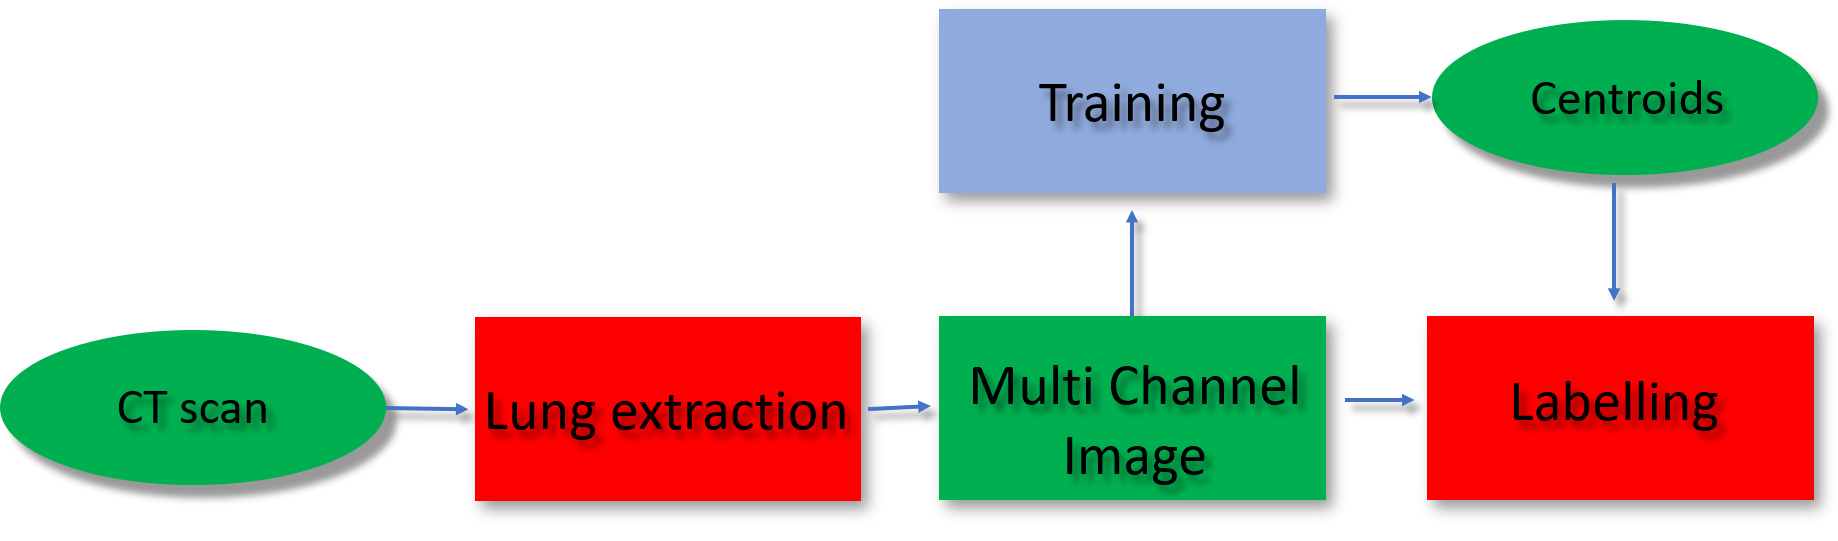
\includegraphics[width=\linewidth]{./img/Pipeline2}
		\begin{columns}
			\begin{column}{.4\textwidth}
				\centering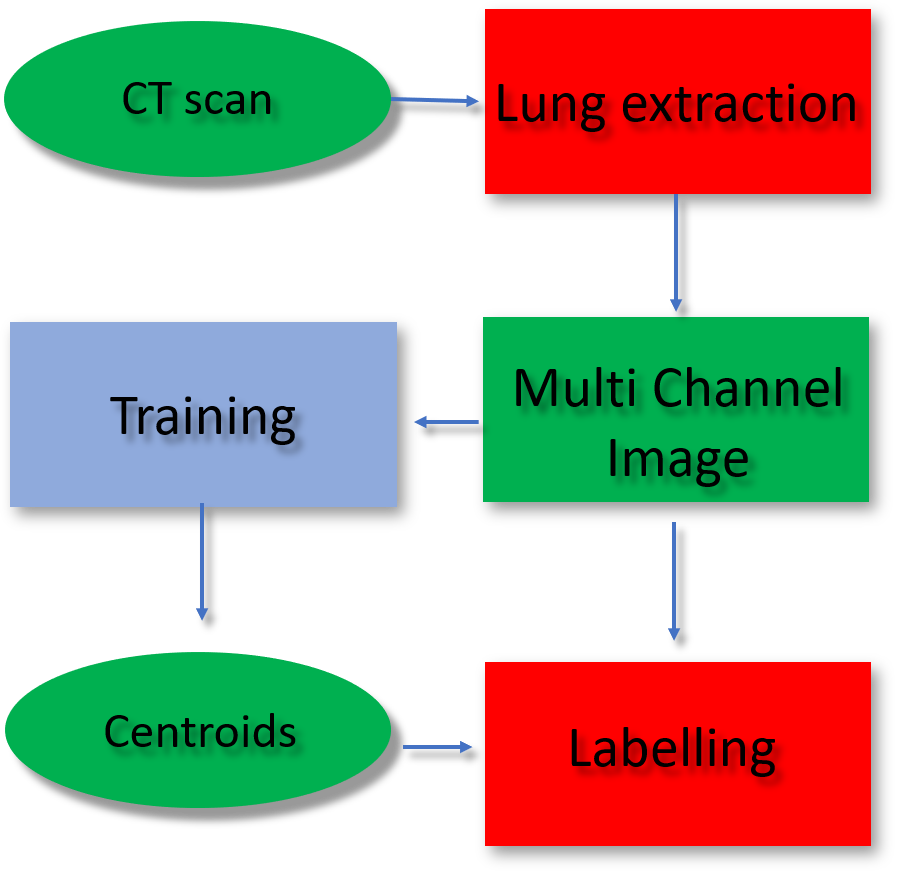
\includegraphics[width=\linewidth]{./img/Pipeline3}
			\end{column}
			\begin{column}{.4\textwidth}
				\begin{block}{}
					\begin{itemize}
						\item \textbf{LANGUAGE:} \textsf{Python} 
\includegraphics[width=.05\textwidth]{./img/python}
						\item \textbf{INSTALLATION:} \textsf{Setup}
						\item \textbf{OS:} Linux 
\includegraphics[width=.05\textwidth]{./img/linux} \&
					Windows 
\includegraphics[width=.05\textwidth]{./img/windows}
						\item \textbf{DOCUMENTATION:} Generated with Sphinx 
\includegraphics[width=.05\textwidth]{./img/sphinx}
						\item \textbf{CI:} Travis 
\includegraphics[width=.05\textwidth]{./img/travis} \& Appveyor 
\includegraphics[width=.05\textwidth]{./img/appveyor}
						\item \textbf{URL:} \url{https://github.com/RiccardoBiondi/segmentation} 
\includegraphics[width=.05\textwidth]{./img/github}
						\item \textbf{DEPENDENCIES:} \textsf{OpenCV} 
\includegraphics[width=.05\textwidth]{./img/OpenCV} \&
						\textsf{SimpleITK} 
\includegraphics[width=.05\textwidth]{./img/simpleitk} \&
						\textsf{Numpy} \includegraphics[width=.05\textwidth]{./img/numpy}
					\end{itemize}
				\end{block}
			\end{column}
		\end{columns}
	\end{frame}
\end{document}